\section{Introduction} 
L’étude des besoins représente une phase fondamentale précédant le développement d’un logiciel. Elle consiste à identifier les fonctionnalités ainsi que les propriétés que le système doit intégrer afin de satisfaire les attentes des utilisateurs. Dans ce chapitre, nous mettrons en évidence les besoins fonctionnels et non fonctionnels dans le but de concevoir une application à la fois performante et fiable. Nous définirons également les principaux acteurs du système et présenterons une vue d’ensemble de l’application, aussi bien sur le plan fonctionnel que technique, avant de terminer par la description de l’architecture adoptée. 

\section{Identification des acteurs} 
Comme évoqué précédemment, notre solution consiste en une plateforme web regroupant différents types d’utilisateurs. Elle fait intervenir plusieurs acteurs principaux, chacun jouant un rôle spécifique dans le fonctionnement du système : 
\begin{itemize}

\item \textbf{Utilisateur} : Cet acteur représente l’utilisateur de base de la plateforme. Il peut consulter l’ensemble des annonces disponibles (animaux à vendre, animaux pour accouplement, animaux en adoption, services animaliers, ainsi que les déclarations de perte et de trouvaille). Il a également la possibilité de gérer son compte personnel, de publier des annonces pour proposer son animal à l’accouplement ou à l’adoption, ainsi que de publier des annonces de perte ou de trouvaille d’animaux.

\item \textbf{Prestataire de service} : Cet acteur hérite de l’acteur \textbf{Utilisateur}. Il peut s’agir d’un dresseur d’animaux, d’un vétérinaire, d’un gardien d’animaux ou d’un toiletteur. En plus des fonctionnalités de base, il peut créer, modifier et gérer ses annonces de services destinés aux animaux afin de proposer ses prestations sur la plateforme.

\item \textbf{Vendeur} : Cet acteur hérite également de l’acteur \textbf{Utilisateur}. Il a la possibilité de mettre en vente des animaux, soit via un système d’enchères, soit à prix fixe. Il peut également gérer ses annonces de vente (ajout, modification, suppression).

\item \textbf{Administrateur} : Il est responsable de la gestion globale de la plateforme. Il peut gérer tous les utilisateurs ainsi que toutes les annonces (vente d’animaux, accouplement, adoption, services et déclarations de perte et de trouvaille). Il dispose également de droits de modération afin de garantir la qualité et la sécurité du contenu publié.

\end{itemize}

\section{Besoins Fonctionnels} 
\subsection{Pour un utilisateur}

Lorsqu’un utilisateur accède à notre plateforme, il peut effectuer les actions suivantes :

\begin{itemize}
    \item S’inscrire et créer un compte.
    \item Consulter l’ensemble du contenu disponible sur la plateforme.
    \item Gérer son compte (modifier ou supprimer ses informations personnelles).
    \item Gérer ses déclarations de perte ou de trouvaille d’animaux (ajouter, modifier, supprimer).
    \item Gérer ses annonces d’animaux destinés à l’accouplement (ajouter, modifier, supprimer).
    \item Gérer ses annonces d’animaux destinés à l’adoption (ajouter, modifier, supprimer).
    \item Gérer ses envois, notamment : demandes d’accouplement, demandes d’adoption, indices liés aux déclarations de trouvaille d’animaux, offres pour les enchères et réservations de services.
    \item Gérer ses réceptions, telles que : intérêts reçus pour l’accouplement, intérêts reçus pour l’adoption et indices reçus concernant les déclarations de trouvaille d’animaux.
\end{itemize} 

\subsection{Pour un vendeur}

Lorsqu’un vendeur accède à notre plateforme, et puisqu’il hérite du rôle d’utilisateur, il dispose de l’ensemble des fonctionnalités offertes à un utilisateur. En plus de cela, il peut également :

\begin{itemize}
    \item Gérer ses animaux à vendre (ajouter, modifier et supprimer), que ce soit à prix fixe ou sous forme d’enchères. 
    \item Gérer les offres reçues pour ses enchères.
    \item Gérer ses produits à vendre (ajouter, modifier et supprimer).
\end{itemize} 


\subsection{Pour un prestataire de service} 
Lorsqu’un prestataire de service accède à notre plateforme,et puisqu’il hérite du rôle d’utilisateur, il dispose de l’ensemble des fonctionnalités offertes à un utilisateur. En plus de cela, il peut également : 
\begin{itemize}
    \item Gérer (ajouter ,modifier , supprimer) ses annonces de service (Véterinaire , dressage , toilettage , garderie ) pour animaux . 
    \item Consulter et gérer les demandes de réservation effectuées par les utilisateurs pour ses services.
\end{itemize} 
\subsection{Pour un administrateur}

Lorsqu’un administrateur accède à la plateforme, il peut effectuer les actions suivantes :

\begin{itemize}
    \item Consulter son tableau de bord et gérer l’ensemble des éléments de la plateforme, notamment : les utilisateurs, les animaux à vendre, les animaux destinés à l’accouplement, les animaux proposés à l’adoption, les services animaliers, ainsi que les déclarations de perte et de trouvaille.
\end{itemize} 

\section{Besoins non fonctionnels}

Dans une architecture distribuée composée de services indépendants, les besoins non fonctionnels sont essentiels pour garantir la qualité, la fiabilité et l’efficacité globale du système. Ils définissent les contraintes que la plateforme doit respecter afin d’assurer une expérience utilisateur optimale et un fonctionnement robuste.

\begin{itemize}

    \item \textbf{Ergonomie et expérience utilisateur} : Proposer une interface simple, intuitive et cohérente, permettant aux utilisateurs de naviguer facilement et d’accéder rapidement aux différentes fonctionnalités. L’objectif est de garantir une expérience fluide, agréable et adaptée à différents supports.

    \item \textbf{Scalabilité} : Assurer la capacité du système à supporter une augmentation progressive ou soudaine du nombre d’utilisateurs et de requêtes, sans dégradation des performances. Chaque composant doit pouvoir évoluer de manière indépendante selon la charge.

    \item \textbf{Disponibilité} : Garantir un accès continu aux services de la plateforme avec un minimum d’interruptions. Le système doit rester fonctionnel même en cas de perturbation partielle de certains composants.

    \item \textbf{Résilience et tolérance aux pannes} : Assurer la continuité du service même en cas de défaillance d’un ou plusieurs composants. Le système doit être capable d’isoler les erreurs et de maintenir les fonctionnalités critiques opérationnelles.

    \item \textbf{Performance} : Optimiser les temps de réponse et assurer un traitement efficace des requêtes, même dans des conditions de forte charge ou de communication entre plusieurs composants.

    \item \textbf{Sécurité} : Protéger les données et contrôler strictement les accès aux différentes fonctionnalités. Le système doit garantir la confidentialité, l’intégrité et la disponibilité des informations échangées.

    \item \textbf{Maintenabilité} : Faciliter l’évolution du système, la correction des anomalies et l’ajout de nouvelles fonctionnalités. Une bonne organisation interne doit permettre des modifications sans impact global sur la plateforme.

    \item \textbf{Observabilité} : Permettre le suivi du comportement global du système afin de détecter rapidement les anomalies, analyser les performances et faciliter le diagnostic des problèmes.

    \item \textbf{Interopérabilité} : Assurer une communication fluide entre les différentes parties du système ainsi qu’avec des services externes, à travers des interfaces bien définies.

\end{itemize}
\section{Diagramme de cas d’utilisation global}  
Nous allons illustrer le fonctionnement de notre solution pour chaque acteur à l’aide d’un diagramme de cas d’utilisation. Ce diagramme permet de représenter les interactions entre les différents acteurs et le système, afin de mieux comprendre leur rôle et leur relation avec la plateforme.

Cette figure présente le diagramme global des cas d’utilisation de notre plateforme : 
\begin{figure}[H]
    \centering
    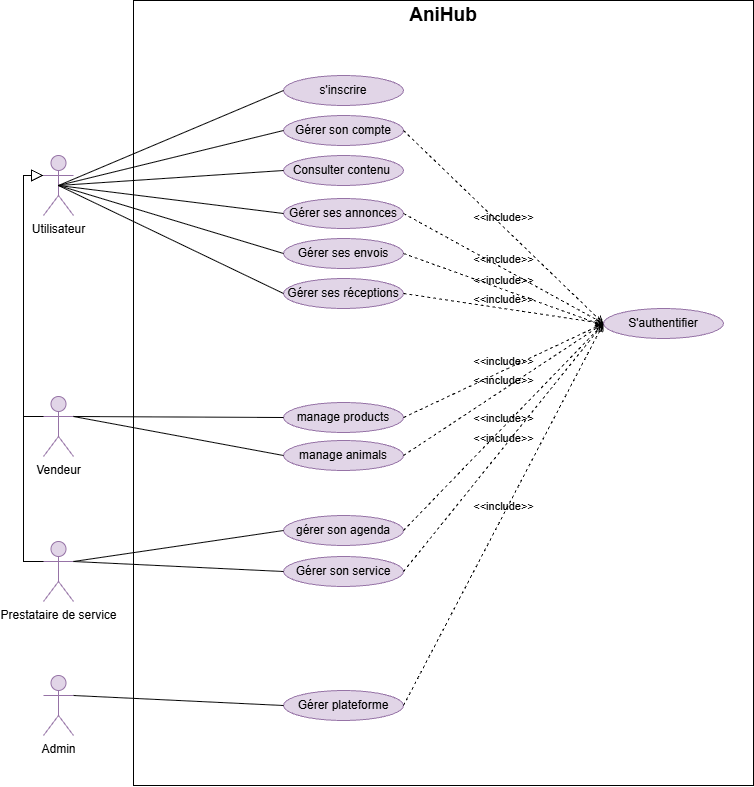
\includegraphics[width=0.94\textwidth]{images/usecase (2).png}
    \caption{Diagramme de cas d'utilisation général}
\end{figure} 
\section{Architecture globale du projet}

Dans cette section, nous présentons l’architecture générale adoptée pour le projet. Nous décrivons d’abord les architectures monolithique et microservices, puis nous les comparons afin de justifier le choix retenu. Enfin, nous détaillons l’architecture globale du système ainsi que ses principaux composants. 
\newpage 
\subsection{Architecture monolithique}

\subsubsection{Principe}
L’architecture monolithique regroupe toutes les fonctionnalités d’une application (interface utilisateur, logique métier et accès aux données) dans une seule unité de déploiement, fortement couplée et exécutée dans un même processus.

\subsubsection{Avantages}
\begin{itemize}
    \item Simplicité de développement et de déploiement.
    \item Facilité de test et de gestion dans les petits projets.
    \item Centralisation du code et des dépendances.
\end{itemize}

\subsubsection{Inconvénients}
\begin{itemize}
    \item Difficulté de maintenance lorsque le système devient complexe.
    \item Faible scalabilité.
    \item Redéploiement complet nécessaire à chaque modification.
\end{itemize}

\subsubsection{Cas d’utilisation}
Cette architecture est adaptée aux petites applications, aux prototypes ou aux projets avec une faible complexité et un nombre limité de fonctionnalités.

\subsection{Architecture microservices}

\subsubsection{Principe}
L’architecture microservices est une approche dans laquelle une application est décomposée en plusieurs services indépendants, chacun responsable d’une fonctionnalité métier spécifique. Chaque service est autonome et communique avec les autres via des API.

\subsubsection{Avantages}
\begin{itemize}
    \item Forte modularité et indépendance des services.
    \item Scalabilité indépendante de chaque composant.
    \item Déploiement et mise à jour sans impacter tout le système.
\end{itemize}

\subsubsection{Inconvénients}
\begin{itemize}
    \item Complexité de gestion et de déploiement.
    \item Communication réseau entre services.
    \item Besoin d’une infrastructure plus avancée.
\end{itemize}

\subsubsection{Cas d’utilisation}
Cette architecture est adaptée aux systèmes complexes, aux plateformes évolutives, aux applications distribuées et aux projets nécessitant une forte scalabilité.
\newpage
\subsection{Comparaison entre architecture monolithique et microservices}

Cette section présente une comparaison entre les architectures monolithique et microservices afin de mettre en évidence leurs principales différences.

La figure ci-dessous illustre le contraste entre une application centralisée et une architecture distribuée en services indépendants.

\begin{figure}[H]
    \centering
    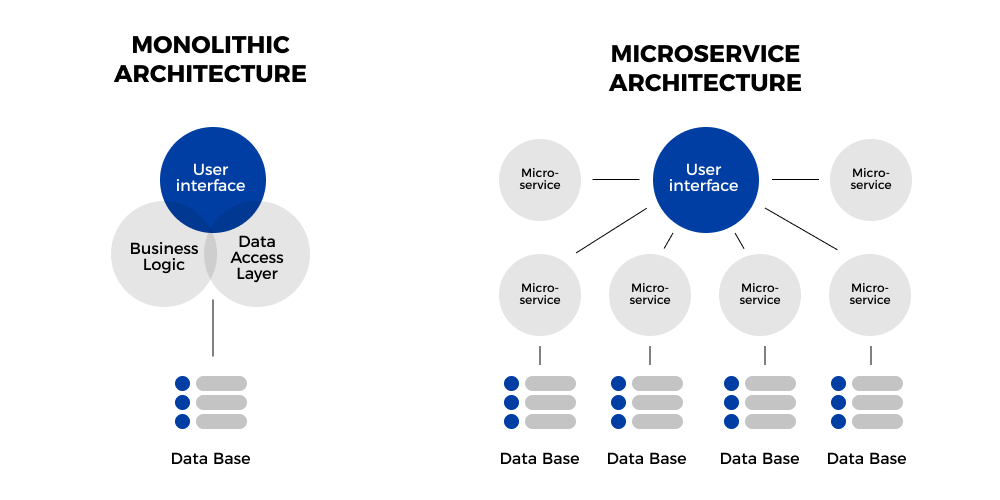
\includegraphics[width=0.9\linewidth]{images/micro vs mono.png}
    \caption{Comparaison architecture monolithique vs microservices}
\end{figure}

Le tableau ci-dessous illustre une comparaison détaillée entre les deux architectures selon plusieurs critères.


\begin{longtable}{|p{3.5cm}|p{6cm}|p{6cm}|}
\hline
\rowcolor{coloranihub}
\textbf{Critères} & \textbf{Architecture monolithique} & \textbf{Architecture microservices} \\
\hline
Structure & Application unique & Services indépendants \\
\hline
Déploiement & Global & Par service \\
\hline
Scalabilité & Limitée & Flexible et fine \\
\hline
Maintenance & Complexe avec la taille & Simplifiée par modularité \\
\hline
Évolution & Impact global & Indépendante par service \\
\hline
Technologies & Homogènes & Hétérogènes possibles \\
\hline
Performance & Adaptée aux petits systèmes & Optimisée pour systèmes distribués \\
\hline
Tolérance aux pannes & Impact global & Isolation des pannes \\
\hline
Complexité & Faible au départ & Plus élevée \\
\hline
Organisation des équipes & Centralisée & Distribuée \\
\hline
\end{longtable}

Ainsi, l’architecture microservices offre une meilleure flexibilité et évolutivité, tandis que l’architecture monolithique reste plus simple à mettre en place pour des systèmes de petite taille.
\subsection{Choix de l’architecture du projet}
\subsubsection{Justification du choix de l’architecture microservices}

Dans notre projet, nous avons opté pour l’architecture microservices pour les raisons suivantes.

\begin{itemize}

\item \textbf{Découpage fonctionnel :} \textbf{"AniHub"} regroupe plusieurs modules indépendants (marketplace, services de bien-être animal, adoption, accouplement, aide à la découverte des animaux perdus). Par exemple, la gestion des annonces d’adoption est indépendante du module marketplace, ce qui justifie une séparation en services. 
\item 
\item \textbf{Évolutivité :} \textbf{"AniHub"} étant une première version évolutive, de nouvelles fonctionnalités telles que le web scraping ou un module d’IA peuvent être ajoutées sans impacter les services existants.

\item \textbf{Résilience :} dans \textbf{"AniHub"}, une panne d’un service comme le module marketplace n’affecte pas les autres fonctionnalités (ex : le module d'accouplement).

\item \textbf{Scalabilité :} certains modules de \textbf{"AniHub"}, tels que le marketplace ou les services de bien-être animal, peuvent être plus sollicités et nécessitent une montée en charge indépendante.
\end{itemize}
\subsubsection{Présentation de notre architecture}

Cette figure illustre la structure générale de l’architecture microservices d’AniHub.

\begin{figure}[H]
    \centering
    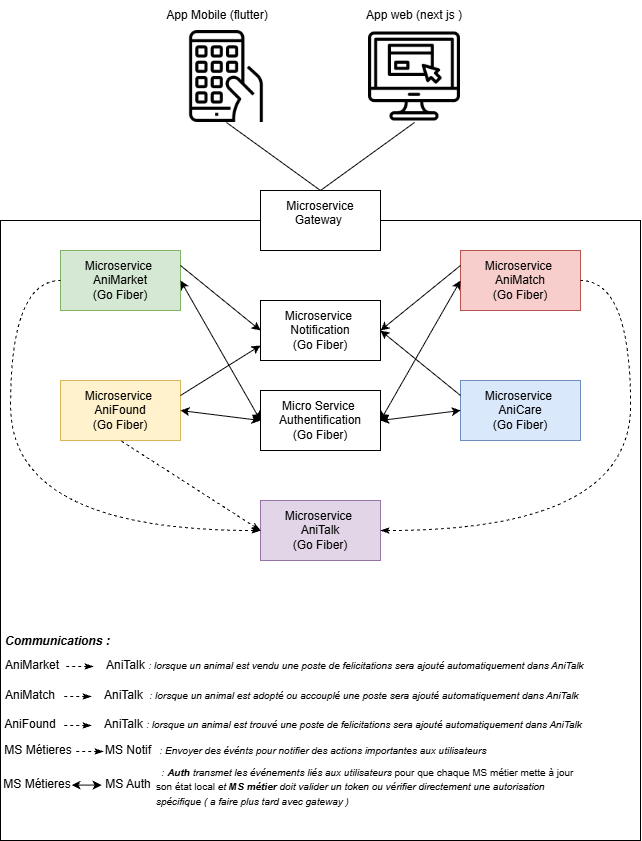
\includegraphics[width=0.5\linewidth]{images/Présentation de notre architecture.png}
    \caption{Présentation de notre architecture}
    \label{fig:arch_anihub}
\end{figure}


Les applications clientes, développées avec \textbf{Next.js} pour le web et \textbf{Flutter} pour le mobile, accèdent au système via un \textbf{API Gateway}, qui assure le routage des requêtes vers les microservices concernés.

\vspace{0.3cm}

L’architecture est composée de plusieurs microservices métiers développés avec \textbf{Go Fiber}, tels que :

\begin{itemize}
    \item \textbf{AniMatch} : gestion de l’adoption et de la mise en relation entre animaux.
    \item \textbf{AniMarket} : marketplace des produits animaliers.
    \item \textbf{AniFound} : gestion des animaux perdus et retrouvés.
    \item \textbf{AniCare} : services et soins animaliers.
    \item \textbf{AniTalk} : espace de communication et d’échanges.
\end{itemize}

\vspace{0.3cm}



\section{Stack technologique et outils de développement} 
\subsection{Outils et environnement de développement}

\subsubsection{Slack}
\begin{center}
    
\includegraphics[width=2cm]{images/slack.png}
\end{center}
Slack est une plateforme de communication collaborative permettant aux équipes de discuter, partager des fichiers et organiser le travail via des canaux dédiés.

\vspace{0.3cm}

\subsubsection{draw.io}
\begin{center}
    
\includegraphics[width=2cm]{images/drawio.png}
\end{center}
draw.io est un outil en ligne permettant de créer facilement des diagrammes tels que les diagrammes UML, les organigrammes et les schémas d’architecture.

\vspace{0.3cm}

\subsubsection{Figma}
\begin{center}
    
\includegraphics[width=1.5cm]{images/figma.png}
\end{center}
Figma est un outil de conception d’interfaces utilisateur (UI/UX) collaboratif, utilisé pour créer des maquettes, prototypes et designs interactifs.

\vspace{0.3cm}

\subsubsection{Visual Studio Code}
\begin{center}
    
\includegraphics[width=2cm]{images/vscode.png}
\end{center}
Visual Studio Code est un éditeur de code source léger et puissant, supportant plusieurs langages de programmation et offrant des extensions pour améliorer la productivité des développeurs.

\vspace{0.3cm}

\subsubsection{Git et GitHub}

\begin{center}
\begin{minipage}{0.45\textwidth}
    \centering
    
\includegraphics[width=2cm]{images/git.png}
    
    \textbf{Git}
\end{minipage}
\hfill
\begin{minipage}{0.45\textwidth}
    \centering
    
\includegraphics[width=2cm]{images/github.png}
    
    \textbf{GitHub}
\end{minipage}
\end{center}

Git est un système de gestion de versions distribué permettant de suivre les modifications du code source, de gérer les différentes versions d’un projet et de faciliter le travail collaboratif entre les développeurs. GitHub est une plateforme d’hébergement de code basée sur Git, offrant des fonctionnalités de collaboration telles que le partage de dépôts, la gestion des versions, le suivi des problèmes (issues) et l’intégration continue.

\subsubsection{GitHub Actions}
\begin{center}
    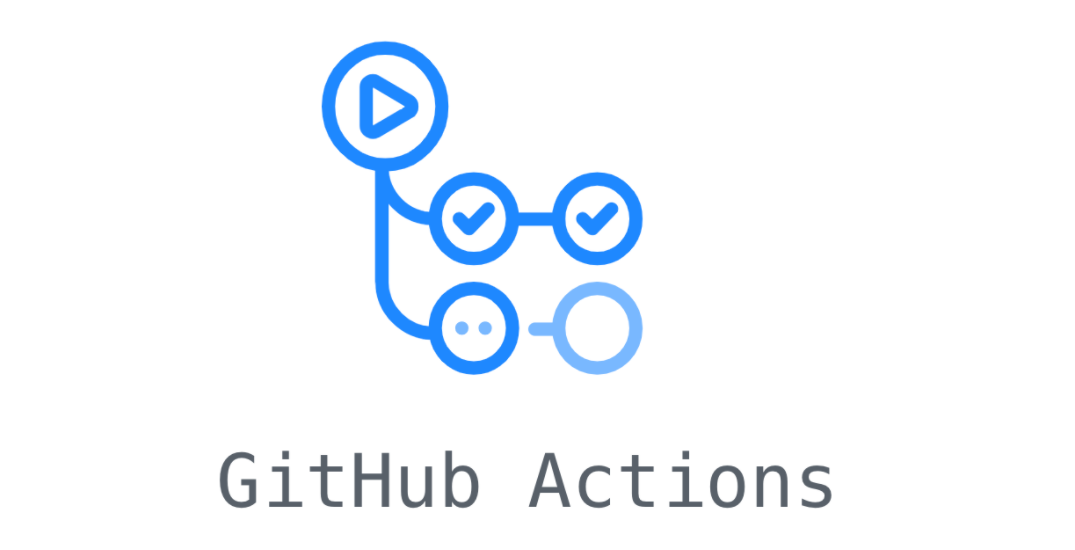
\includegraphics[width=7cm]{images/githubActions.png}
\end{center} 


GitHub Actions est un outil d’intégration et de déploiement continu (CI/CD) permettant d’automatiser les tâches de build, de test et de déploiement des applications directement depuis les dépôts GitHub.


\subsection{Stack technologique}

\subsubsection{TypeScript}
\begin{center}
    
\includegraphics[width=2cm]{images/typescript.png}
\end{center}
TypeScript est un langage de programmation basé sur JavaScript qui ajoute le typage statique, permettant de rendre le code plus robuste, maintenable et moins sujet aux erreurs.

\vspace{0.3cm}

\subsubsection{Next.js}
\begin{center}
    
\includegraphics[width=2cm]{images/nextjs.png}
\end{center}
Next.js est un framework basé sur React permettant de développer des applications web modernes avec rendu côté serveur (SSR), génération statique (SSG) et optimisation des performances.

\vspace{0.3cm}

\subsubsection{Tailwind CSS}
\begin{center}
    
\includegraphics[width=2.7cm]{images/tailwind.png}
\end{center}
Tailwind CSS est un framework CSS utilitaire permettant de concevoir rapidement des interfaces modernes et responsives sans écrire de CSS personnalisé complexe.

\vspace{0.3cm}

\subsubsection{Go et Fiber}

\begin{center}
\begin{minipage}{0.45\textwidth}
    \centering
    
\includegraphics[width=3cm]{images/go.png}
    
\end{minipage}
\hfill
\begin{minipage}{0.45\textwidth}
    \centering
    
\includegraphics[width=3cm]{images/fiber.png}
    
\end{minipage}
\end{center}

Go est un langage de programmation compilé développé par Google, reconnu pour sa simplicité, sa performance et sa gestion efficace de la concurrence. Fiber est un framework web rapide pour Go, inspiré d’Express.js, facilitant la création d’API performantes et légères. 

\subsubsection{Neon PostgreSQL}
\begin{center}
    
\includegraphics[width=3cm]{images/neon.jpg}
\end{center}
Neon PostgreSQL est une plateforme de base de données serverless basée sur PostgreSQL, offrant scalabilité, performance et séparation du stockage et du calcul.

\vspace{0.3cm} 


 \subsubsection{Postman}

\begin{center}
    
\includegraphics[width=4cm]{images/postman.png}
\end{center}

Postman est un outil de test et de développement d’API permettant d’envoyer des requêtes HTTP, de vérifier les réponses des services et de faciliter le débogage des interfaces backend.

\subsubsection{RabbitMQ}

\begin{center}
    
\includegraphics[width=4cm]{images/rabbit.png}
\end{center} 



RabbitMQ est un système de messagerie (message broker) permettant la communication asynchrone entre les différents services d’une architecture distribuée. Il facilite l’échange de messages entre producteurs et consommateurs afin d’assurer un découplage des composants, une meilleure scalabilité et une gestion efficace des traitements en arrière-plan. 
\subsubsection{Docker}
\begin{center}
    
\includegraphics[width=3.4cm]{images/docker.png}
\end{center}
Docker est une plateforme de conteneurisation permettant d’emballer les applications et leurs dépendances afin d’assurer leur portabilité et leur déploiement rapide.

\vspace{0.3cm}

\subsubsection{Kubernetes}
\begin{center}
    
\includegraphics[width=2.8cm]{images/k8s.png}
\end{center}
Kubernetes est un système d’orchestration de conteneurs permettant de déployer, gérer et scaler automatiquement des applications conteneurisées. 

\section{Pilotage du projet : méthode Scrum} 
Comme mentionné précédemment, la méthodologie Scrum a été retenue pour ce projet. 
\subsection{Équipe et rôles} 
La figure ci-dessous illustre les différentes parties prenantes de l’application : 
\begin{figure}[H]
    \centering
    
\includegraphics[width=0.92\linewidth]{images/scrumteam.png}
    \caption{Équipe et rôles Scrum}
\end{figure}\newpage 





\subsection{Backlog produit} 
Le backlog Scrum regroupe les user stories priorisées du projet. Le tableau ci-dessous présente le backlog produit.
\begin{longtable}{|p{4cm}|p{9.5cm}|p{2cm}|} 
\caption{Backlog produit}\label{tab:product-backlog}\\
\hline
\rowcolor{coloranihub}
\textbf{Product Backlog Item (Sprint)} & \textbf{User Story} & \textbf{Priorité} \\
\hline
\endfirsthead

\hline
\rowcolor{coloranihub}
\textbf{Product Backlog Item (Sprint)} & \textbf{User Story} & \textbf{Priorité} \\
\hline
\endhead

\hline
\endfoot

\multirow{5}{4cm}{\textbf{Sprint 1 : Authentification et administration}} 
& En tant qu'utilisateur, je veux accéder à une interface moderne et intuitive, afin de naviguer facilement sur AniHub. & Must Have \\
\cline{2-3}
& En tant qu'utilisateur, je veux créer un compte et me connecter afin d'accéder à la plateforme & Must Have \\
\cline{2-3}
& En tant qu'utilisateur, je veux gérer mon profil afin de personnaliser mes informations & Should Have \\
\cline{2-3}
& En tant qu'administrateur, je veux gérer tous les utilisateurs afin de superviser la plateforme & Must Have \\
\cline{2-3}
& En tant qu'administrateur, je veux gérer toutes les annonces (animaux, déclarations, services) afin de superviser et contrôler le contenu de la plateforme & Must Have \\
\hline
% ===================== SPRINT 2ANIMATCH=====================
\multirow{9}{4cm}{\textbf{Sprint 2 : Module AniMatch}}
& En tant qu’utilisateur, je veux consulter la liste des animaux (adoption ou accouplement) afin de trouver un partenaire compatible & Must Have \\
\cline{2-3}
& En tant qu’utilisateur, je veux gérer mes annonces afin de les publier, modifier et supprimer. & Must Have \\
\cline{2-3}
& En tant qu’utilisateu,je veux gérer mes invitations envoyées pour suivre mes interactions, publier , modifier ou annuler une demande d'adoption ou accouplement & Must Have \\
\cline{2-3}
& En tant qu’utilisateur, je veux gérer les invitations reçues pour adoption ou accouplement afin de répondre aux demandes, accepter ou refuser les propositions et organiser mes interactions. & Must Have \\
\cline{2-3}
& En tant qu'utilisateur, je veux gérer mes notifications afin d’être informé en temps réel des interactions liées à mes annonces et activités sur \textbf{AniMatch} & Should Have \\
\cline{2-3}
& En tant qu'utilisateur, je veux discuter avec un autre propriétaire afin de finaliser une adoption ou un accouplement & Should Have \\
\hline
% ===================== SPRINT 3 : ANIFOUND =====================
\multirow{8}{4cm}{\textbf{Sprint 3 : Module AniFound}}
& En tant qu’utilisateur, je souhaite consulter les déclarations de perte et de trouvaille afin de retrouver ou identifier un animal & Must Have \\
\cline{2-3}
& En tant qu'utilisateur, je veux gérer mes déclarations de perte (modifier/supprimer) afin de mettre à jour mes informations & Must Have \\
\cline{2-3}
& En tant qu’utilisateur, je veux envoyer, gérer, modifier, annuler et suivre le statut de mes indices afin de prouver qu’il s’agit bien de mon animal. & Must Have \\
\cline{2-3}
& En tant qu’utilisateur, je veux gérer les indices reçus afin de les examiner et d’y répondre (acceptation ou refus) & Must Have \\
\cline{2-3}
& En tant qu’utilisateur, je veux gérer mes notifications afin d’être informé des interactions sur mes déclarations de perte, de trouvaille et de mes indices. & Should Have \\
\cline{2-3}
& En tant qu’utilisateur, je veux contacter l’autre partie afin d’échanger des informations et faciliter la résolution de la situation & Should Have \\
\hline
% ===================== SPRINT 4 : ANIMARKET =====================
\multirow{10}{4cm}{\textbf{Sprint 4 : Module AniMarket}}
&En tant qu’utilisateur, je veux consulter la liste des animaux à vendre afin de découvrir les annonces disponibles et comparer les différentes offres proposée & Must Have \\
\cline{2-3}

& En tant qu’utilisateur, je veux proposer une offre sur une enchère afin de participer au processus d’achat et tenter d’acquérir un animal & Must Have \\
\cline{2-3}

& En tant qu’utilisateur, je veux gérer mes notifications afin d’être informé des interactions sur mes annonces et activités (offres, enchères, wishlist) et suivre les mises à jour en temps réel & Should Have \\
\cline{2-3}

& En tant que vendeur, je veux gérer mes animaux à vendre afin de maintenir mes annonces à jour, les publier, les modifier ou les supprimer selon leur disponibilité & Must Have \\
\cline{2-3}
& En tant que vendeur, je veux gérer les offres reçues afin de les consulter, les accepter ou les refuser selon les propositions des acheteurs  & Must Have \\
\cline{2-3}

& En tant qu’utilisateur, je veux commenter et noter un animal afin de partager mon avis et évaluer les annonces consultées  & Could Have \\
\cline{2-3}

& En tant qu’utilisateur, je veux discuter avec le vendeur afin d’échanger des informations complémentaires et faciliter la transaction  & Should Have \\
\hline
% ===================== SPRINT 5 : ANICARE =====================
\multirow{8}{4cm}{\textbf{Sprint 5 : Module AniCare}}
& En tant qu’utilisateur, je souhaite consulter la liste des services afin de découvrir les services disponibles et choisir celui qui correspond le mieux à mes besoins & Must Have \\
\cline{2-3}

& En tant qu’utilisateur, je souhaite gérer mes réservations envoyées (envoyer, suivre, modifier, annuler) afin de gérer efficacement mes demandes & Must Have \\
\cline{2-3}

& En tant qu’utilisateur, je souhaite gérer mes notifications afin d’être informé des interactions sur mes activités & Should Have \\
\cline{2-3}

& En tant qu’utilisateur, je souhaite discuter avec l’autre partie (utilisateur ou prestataire) afin de faciliter la communication & Should Have \\
\cline{2-3}

& En tant que prestataire de service, je souhaite gérer mon propre service (publier, mettre à jour, supprimer) afin de présenter mes services de manière claire & Must Have \\
\cline{2-3}

& En tant que prestataire de service, je souhaite gérer mes réservations reçues afin de répondre aux demandes des clients et organiser efficacement mes prestations & Must Have \\
\cline{2-3}

& En tant que prestataire de service, je souhaite gérer mes cours afin de les organiser, les publier et les mettre à jour selon mes besoins & Won’t Have \\
\cline{2-3}

& En tant qu’utilisateur, je souhaite consulter les cours des prestataires de service afin de découvrir les contenus disponibles et apprendre selon mes besoins & Won’t Have \\
\hline 

% ===================== SPRINT 6 : DEVOPS =====================
\multirow{4}{4cm}{\textbf{Sprint 6 : Conteneurisation, CI/CD, Déploiement Cloud et Monitoring}}
& Conteneuriser les microservices avec Docker afin de garantir un environnement d’exécution stable et portable & Must Have \\
\cline{2-3}
& Déployer les microservices sur Kubernetes afin d’assurer l’orchestration et la disponibilité de l’application. & Must Have \\
\cline{2-3}
& Déployer l’application sur Google Cloud Platform (GCP) afin de rendre la plateforme accessible en ligne. & Must Have \\
\cline{2-3}
& Automatiser le build et le déploiement avec GitHub Actions afin d’assurer un processus CI/CD rapide et fiable. & Should Have \\  
\cline{2-3}
& Surveiller les microservices avec Grafana afin de suivre les performances et détecter les anomalies du système. & Could Have \\
\hline


\end{longtable} 


\subsection{Méthode de priorisation MoSCoW}

La priorisation des besoins est réalisée selon la méthode MoSCoW. Le tableau ci-dessous illustre les différentes catégories de cette méthode : 


\definecolor{coloranihub}{HTML}{E1D5E7}

\begin{longtable}{|p{3.5cm}|p{12cm}|}
\caption{Catégories de la méthode MoSCoW}
\label{tab:moscow} \\
\hline
\rowcolor{coloranihub}
\textbf{Catégorie} & \textbf{Description} \\
\hline
\endfirsthead

\hline
\rowcolor{coloranihub}
\textbf{Catégorie} & \textbf{Description} \\
\hline
\endhead

\textbf{Must Have} & Fonctionnalités essentielles au bon fonctionnement du système, sans lesquelles le produit ne peut pas fonctionner correctement. \\
\hline

\textbf{Should Have} & Fonctionnalités importantes mais non essentielles. Elles améliorent le système, sans être indispensables à son fonctionnement. \\
\hline

\textbf{Could Have} & IFonctionnalités optionnelles qui améliorent l’expérience utilisateur, sans être nécessaires dans la première version. \\
\hline

\textbf{Won’t Have} & Fonctionnalités non retenues pour cette version du projet, en raison de contraintes de temps, de ressources ou de priorité. \\
\hline

\end{longtable}

\newpage
\subsection{Planification des sprints et des releases}

Le tableau ci-dessous présente la planification des sprints ainsi que des releases du projet : 

\renewcommand{\arraystretch}{1.5}

\begin{longtable}{|m{4cm}|m{4cm}|m{6cm}|>{\centering\arraybackslash}m{2cm}|}
\caption{Planification des sprints et des releases} \\
\hline
\rowcolor{coloranihub}
\textbf{Release} & \textbf{Sprint} & \textbf{Description} & \textbf{Durée} \\
\hline
\endfirsthead

\hline
\rowcolor{coloranihub}
\textbf{Release} & \textbf{Sprint} & \textbf{Description} & \textbf{Durée} \\
\hline
\endhead

\multirow{3}{4cm}{\textbf{Release 1 : AniHub partie 1}} 
& Sprint 1 : Authentification et Administration 
& Gestion de l’inscription, de la connexion, des rôles ainsi que du tableau de bord administrateur 
& 2 semaines \\
\cline{2-4}

& Sprint 2 : AniMatch 
& Module dédié à la mise en relation pour l’adoption et l’accouplement des animaux 
& 3 semaines \\
\cline{2-4}

& Sprint 3 : AniFound 
& Module permettant la déclaration et la recherche des animaux perdus 
& 3 semaines \\
\hline

\multirow{3}{4cm}{\textbf{Release 2 : AniHub partie 2}} 
& Sprint 4 : AniMarket 
& Gestion des annonces de vente de produits et services liés aux animaux 
& 3 semaines \\
\cline{2-4}

& Sprint 5 : AniCare 
& Gestion des services de soins et du suivi des animaux 
& 3 semaines \\
\cline{2-4}

& Sprint 6 : Conteneurisation, CI/CD, Déploiement et Monitoring 
& Phase de déploiement de l’application, tests finaux et correction des anomalies 
& 2 semaines \\
\hline

\end{longtable} 
\section{Conclusion}

Dans ce chapitre, nous avons présenté l’étude des besoins de la plateforme \textbf{AniHub}, les différents acteurs ainsi que les besoins fonctionnels et non fonctionnels du système. Nous avons également présenté l’architecture microservices adoptée, les technologies utilisées ainsi que l’organisation du projet selon la méthode Scrum, incluant le backlog produit, la planification des sprints et des releases. Cette étude constitue une base essentielle pour la conception et la réalisation de notre application. 

